\chapter{Case Study: Community Detection}\label{chap:2}
In the following chapter we discuss the applicability of our method to community detection problem, which is one of the central problems in network science \cite{Fortunato2010}. The problem initially came from sociology, where a social community is deemed to have more connections between its members, than to the rest of the population. Thus, loosely speaking, a \textit{community}  in a network $G=(V,E)$ is a set of nodes, which are relatively more connected between each other than to the rest of the network. Due to different language in different fields of science, the communities are sometimes referred to as \textit{clusters}. The problem is to find an optimal division of the network into the clusters, which in relation to the graph partitioning problem, is NP-hard. Therefore, we have only approximate algorithms with different ratio of precision vs. computational speed.

However, another problem related to the communities is that they are not precisely defined mathematically. Therefore there exist a vast number of community definitions: as non- or overlapping sets of nodes, multilevel communities (smaller communities inside larger communities), multiplex communities, etc. In this chapter we concentrate on the communities in undirected networks, defined as a partitioning of a node set into non-overlapping subsets of nodes $C=[c_1,c_2, \dots, c_k ]$, such that the number of links between inside each $c_i$ is maximized and between any pair $(c_i, c_j)$ is minimized. Hence, the precise objective function to be optimised during the partitioning is the so-called \textit{modularity} \cite{MN2}. For a network on $n$ nodes with an adjacency matrix $A = (A_{ij})_{i,j=1,..,n}$  the \textit{modularity} of the partition $C$ of a is defined as follows:
$$Q = \frac{1}{2m}\sum\limits_{ij}\left(A_{ij} - \frac{k_i k_j}{2m}\right)\delta(c_i,c_j),$$
where $m$ is the number of edges, $k_i$ is the degree of node $i$ and $\delta$ is the Kronecker delta function. In simple words, the quantity $Q$ compares the current connectivity within groups $C$ with the randomized null model, or what we expect on the average. 

\subsection{Stochastic Block Model}

One network model designed specifically to assess the community detection algorithms is called the \textit{Stochastic Block Model} (SBM) \cite{Abbe2018}. It is sometimes referred to as a \textit{planted partition model} and is defined as follows. Let us have $n$ nodes divided into clusters $C=[c_1,c_2,\dots ,c_k]$ and let us define an affinity matrix of probabilities $B=(b_{ij})_{i,j=1,..,k}$, where  $b_{ij}$ is the node connection probability between groups $i$ and $j$. Then, the graph is generated in a way that resembles the Erdos-Renyi random graph - each pair of nodes from communities $c_i$ and $c_j$ is connected independently of each other with probability $b_{ij}$, where $1\leq i,j\leq k$. On Figure \ref{fig:sbm_example} we show a sample from the SBM model with 3 planted communities. Due to its relative simplicity, this model has become for studying various central questions in machine learning, computer science and statistics \cite{Moore2017}. 

 \begin{figure}[ht]
 \centering
    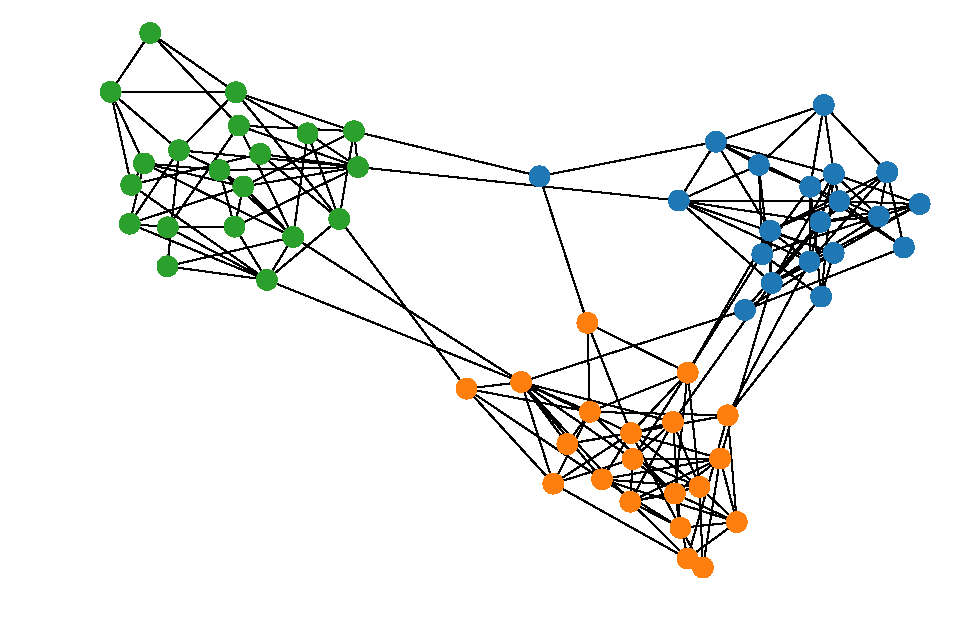
\includegraphics[width=0.7\textwidth]{SBM_example_3clusters.pdf}
   \caption{Example of the stochastic block model with 3 communities}
   \label{fig:sbm_example}
 \end{figure}

The general inference technique, or model fitting procedure, is based on Maximum Likelihood Estimation (MLE). However, even for this simple model there in no exact solution of MLE and computation of the maximum in general case is NP-hard. There exist a number of approximate method based on various optimization algorithms, Monte-Carlo sampling or Bayesian approach \cite{BrianNewman2011}. In the framework of this study we use the MLE estimator given in \cite{Peixoto2014}. 

It is evident that if the connection probabilities are close to each other, the SBM network will resemble the ordinary Erdos-Renyi network. In fact, for the case of SBM with two clusters there exists the detectability threshold given in the following Theorem.
\begin{theorem}\label{thm.detectability_SBM}
The SBM with $n$ nodes and two clusters with symmetric affinity matrix $B$, where $b_{11}=b_{22}=p/n$ and $b_{12}=b_{12}=q/n$, can be inferred with high probability iff $(p-q)^2> 2(p+q)$. When $(p-q)^2 < 2(p+q)$, any algorithm will fail to infer the original SBM with high probability. 
\end{theorem}

In the following subsection we describe the community detection methods used in our study.

\subsection{Community detection methods}

\subsubsection{Greedy modularity maximization}
\subsubsection{Louvain method}
\subsubsection{Infomap}

\subsubsection{Node2Vec + K-means}
We apply our method to the problem of community detection in networks. The node2vec algorithm gives the embedding of the graph into the real space $\mathbb{R}^d$, such that the nodes which are close to each other in the graph are mapped to the close points in the embedding space. Hence, the clustering of nodes can be obtained by any vector clustering algorithm and for our study we used the \textit{k-means clustering} \cite{Macqueen1967}. The choice of the optimal number of cluster is then deduced using \textit{silhouette analysis}. Silhouette analysis can be used to study the separation distance between the resulting clusters. The silhouette plot displays a measure of how close each point in one cluster is to points in the neighboring clusters and thus provides a way to assess parameters like number of clusters visually. This measure has a range of $[-1, 1]$.

Silhouette coefficients (as these values are referred to as) near $+1$ indicate that the sample is far away from the neighboring clusters. A value of $0$ indicates that the sample is on or very close to the decision boundary between two neighboring clusters and negative values indicate that those samples might have been assigned to the wrong cluster. We use the average silhouette score for a clustering to measure its fitness and choose a partition with the largest average score. 

On Figure \ref{fig:silhouette_example} we show the example of the silhouette coefficient calculation for the case of the SBM with four planted clusters. The upper plots show the silhouette scores for the nodes in the assigned cluster by k-means algorithms, dashed red line denotes the average silhouette coefficient of the partitioning. The lower set of plots show the t-SNE two dimensional embedding of the node2vec embedding of the graph nodes. We may notice that cluster structure is well pronounced. 
 \begin{figure}[ht]
 \centering
    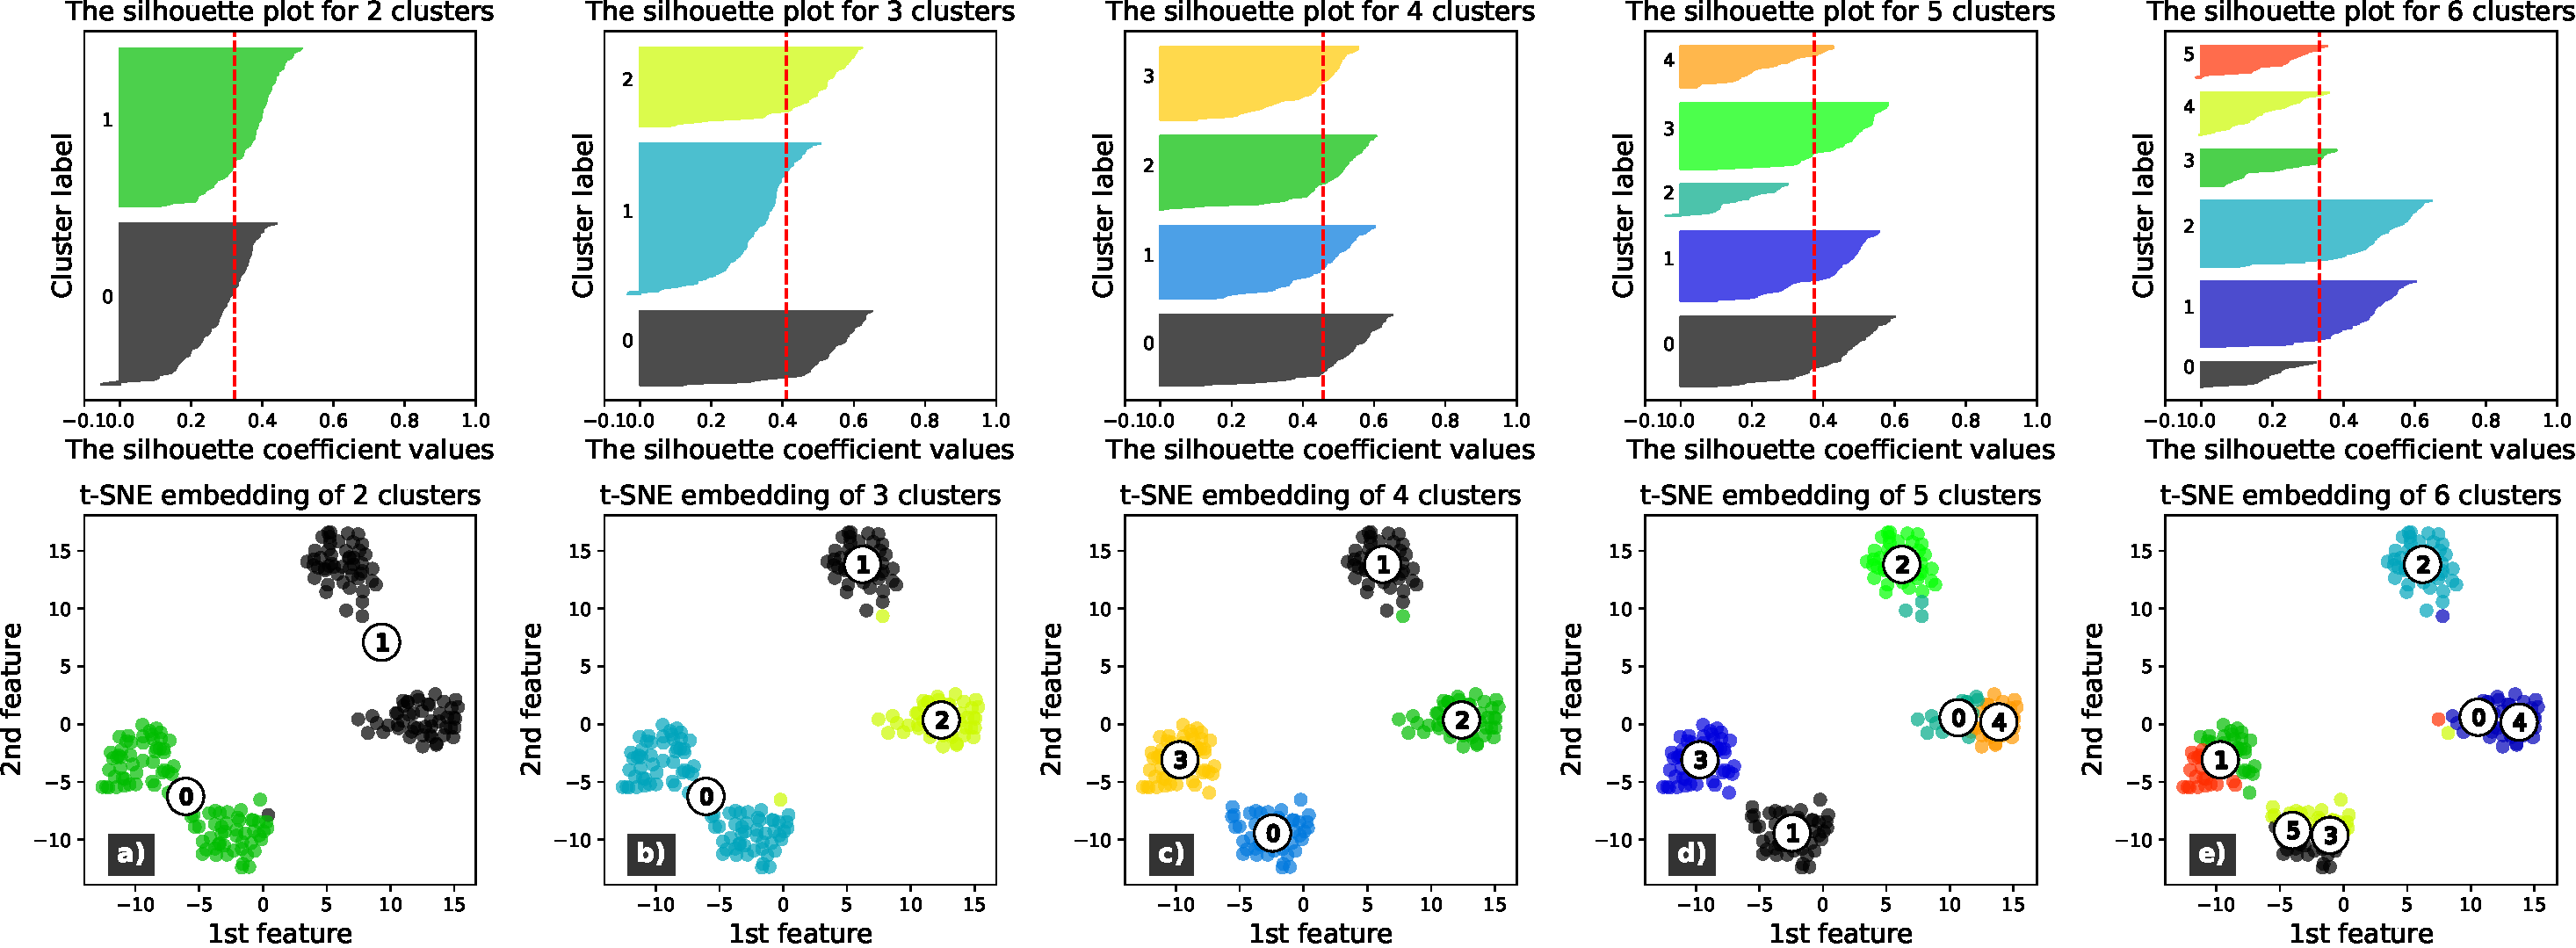
\includegraphics[width=1\textwidth]{avg_silhouette_with_4_clusters_50.pdf}
   \caption{Silhouette plot and t-SNE representation of the embedding for SBM with 4 clusters and inference from a) two to e) six clusters. Red line denotes the average silhouette coefficient.}
   \label{fig:silhouette_example}
 \end{figure}


\section{Comparison of the clustering algorithms}
In this section we compare the performance of clustering algorithms
 \begin{figure}[ht]
 \centering
    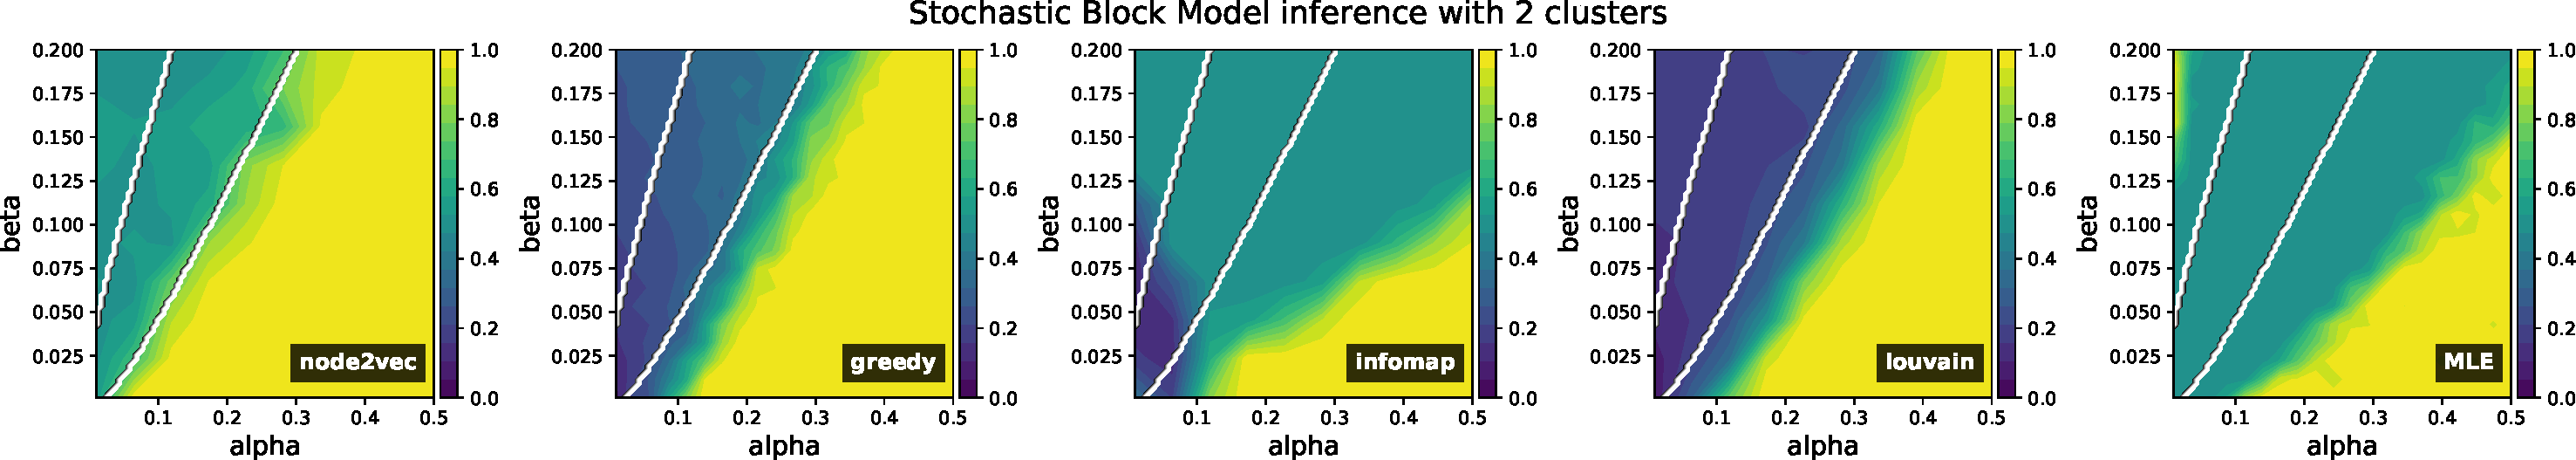
\includegraphics[width=1\textwidth]{clustering_SBM_heatmap_2_clusters.pdf}
   \caption{Comparison of the accuracies of community detection algorithms for symmetric SBM with 2 clusters over a range of $\alpha$ and $\beta$.}
   \label{fig:comparison_clustering_2clusters}
 \end{figure}
 
 \begin{figure}[ht]
 \centering
    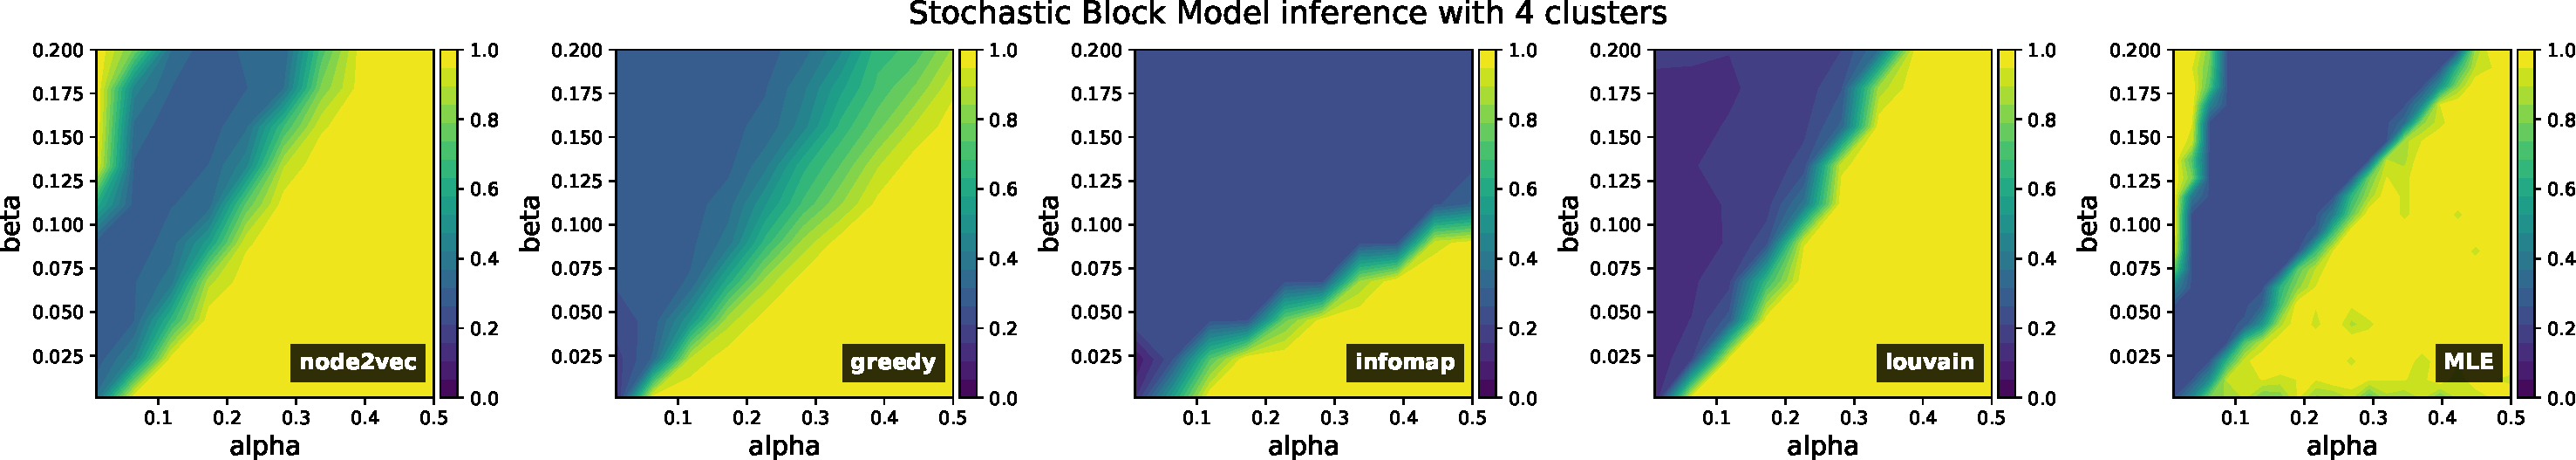
\includegraphics[width=1\textwidth]{clustering_SBM_heatmap_4_clusters.pdf}
   \caption{Comparison of the accuracies of community detection algorithms for symmetric SBM with 4 clusters over a range of $\alpha$ and $\beta$.}
   \label{fig:comparison_clustering_4clusters}
 \end{figure}
 
  \begin{figure}[ht]
 \centering
    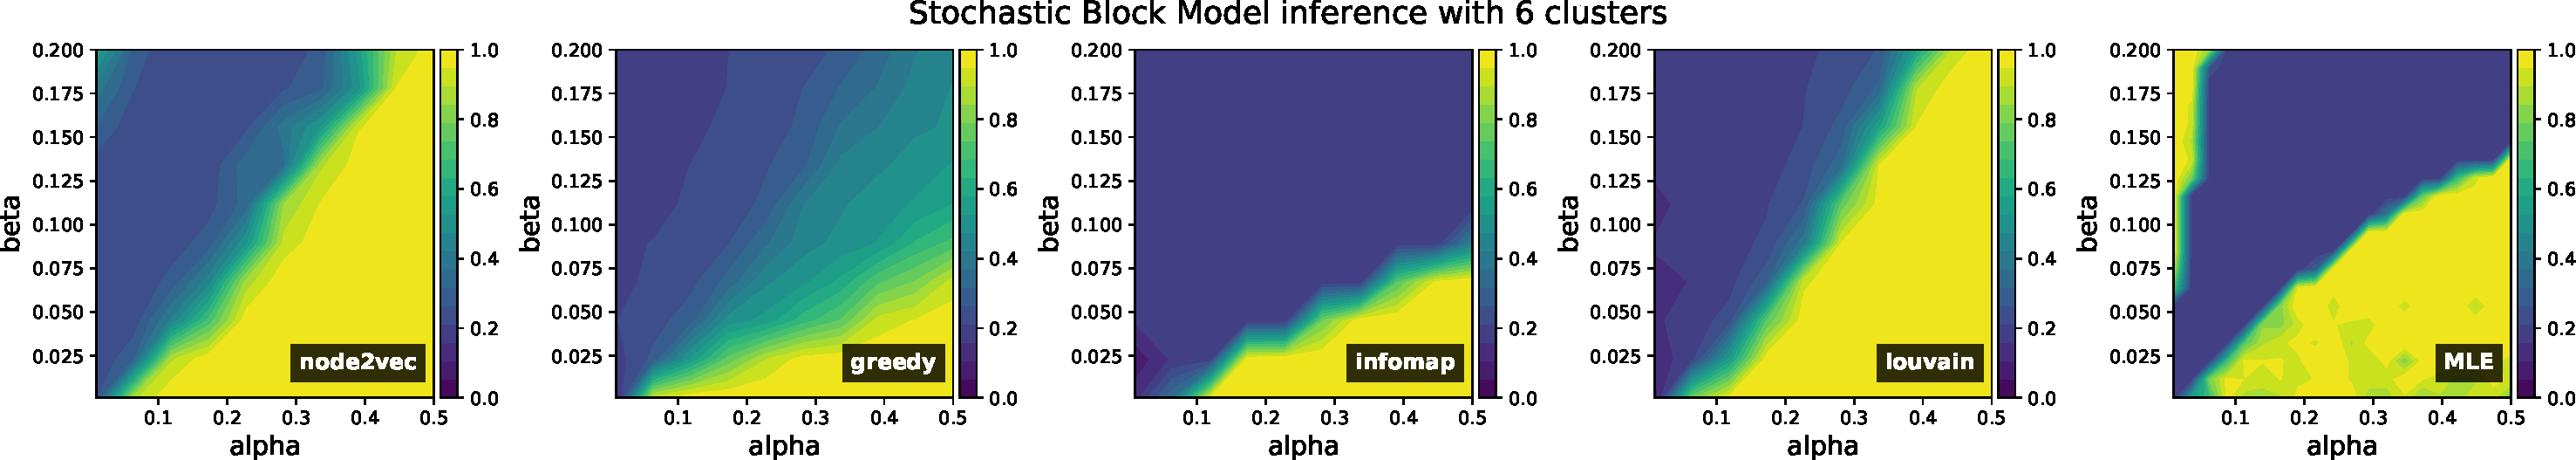
\includegraphics[width=1\textwidth]{clustering_SBM_heatmap_6_clusters.pdf}
   \caption{Comparison of the accuracies of community detection algorithms for symmetric SBM with 6 clusters over a range of $\alpha$ and $\beta$.}
   \label{fig:comparison_clustering_6clusters}
 \end{figure}



\section{Distance Matrix Transformation}
What happened to distance matrix in the graph and after
%
%\begin{figure}[ht]
%\centering
%\begin{minipage}[b]{0.49\textwidth}
%\centering
%\includegraphics[scale=0.6]{av_deg_vs_tau_both_BA.pdf}
%\caption*{Barabasi-Albert network}
%\end{minipage}\hfill
%\begin{minipage}[b]{0.49\textwidth}
%\centering
%\includegraphics[scale=0.6]{av_deg_vs_tau_both_ER.pdf}
%\caption*{Erdos-Renyi network}
%\end{minipage}

% \begin{figure}[ht]
% \centering
%   % \includegraphics[width=0.8*\textwidth]{  }
% 
%   \caption{Figure}
%   \label{fig:}
% \end{figure}

\section{Findings and Hypothesis}
Correlation between embedded information loss and Node Degree?)

